\documentclass{article}
\usepackage[utf8]{inputenc}
\usepackage{hyperref}
\usepackage[letterpaper, portrait, margin=1in]{geometry}
\usepackage{enumitem}
\usepackage{amsmath}
\usepackage{booktabs}
\usepackage{graphicx}
\usepackage{float}

\usepackage{hyperref}
\hypersetup{
colorlinks=true,
    linkcolor=black,
    filecolor=black,      
    urlcolor=blue,
    citecolor=black,
}
\usepackage{natbib}

\usepackage{titlesec}
  
\title{Homework 4}
\author{Lin Yang}
\date{\today}
  
\begin{document}
\maketitle  
\section{Python}
~\\
1. Visually inspect the bycatch by month before and after treatment for treated and control groups by creating a line plot for months in 2017 and 2018. 
\begin{figure}[ht]
\centering
	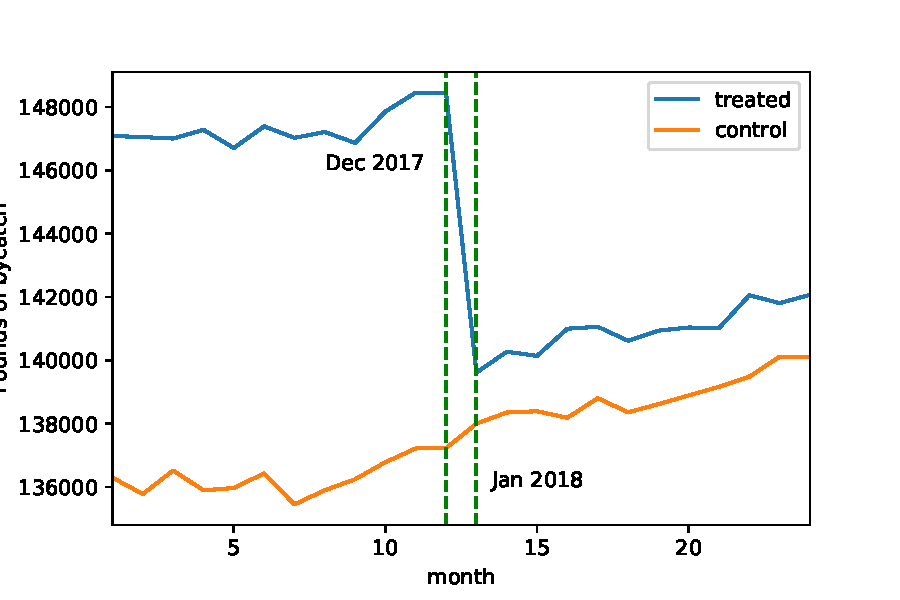
\includegraphics[scale = 0.9]{hw4a.pdf}
    \caption{Monthly amount of bycatch treated group versus control group}
\end{figure}

There exists parallel trend before treatment among treated and control group. 

~\\
2. By following the formula to calculate, the after/before difference of average amount of bycatch for the treatment group is 9591.35 less than the after/before difference for the control group. 

~\\
3.(a) By using the regression-based two-period estimation method, I got the same treatment effects: -9591.35 with the result from question 2. The estimation result is shown in table1 below.
\begin{table}[H]
	\centering
	\begin{tabular}{ll}
\toprule
{} & Coefficients \\
{} &       (s.d.) \\
\midrule
constant        &    138001.81 \\
                &   (18657.80) \\
pre-period      &      -773.22 \\
                &     (598.69) \\
treatment group &     11202.04 \\
                &   (23502.90) \\
treated         &     -9591.35 \\
                &    (3231.79) \\
observations    &          100 \\
\bottomrule
\end{tabular}
	
	\caption{Coefficients and standard errors using Dec 2017 and Jan 2018}
\end{table}

~\\(b) The treatment effect change to -8956.78. And there is a clear difference for the month-indicator variables such that the coefficients for the months before Jan 2018 are negative, and the coefficients for the months after Jan 2018 are positive. The whole estimation results are shown in table 2 (page 4). 
\begin{table}[ht]
	\centering
	\begin{tabular}{ll}
\toprule
{} & Coefficients \\
{} &       (s.d.) \\
\midrule
constant        &    137739.93 \\
                &   (18611.19) \\
treatment group &     11052.45 \\
                &   (23162.97) \\
treated         &     -8956.78 \\
                &    (3166.92) \\
Jan 2017        &     -1585.88 \\
                &     (539.64) \\
Feb 2017        &     -1843.19 \\
                &     (500.22) \\
Mar 2017        &     -1524.83 \\
                &     (514.58) \\
Apr 2017        &     -1667.35 \\
                &     (516.65) \\
May 2017        &     -1941.17 \\
                &     (556.74) \\
June 2017       &     -1359.77 \\
                &     (592.42) \\
July 2017       &     -2007.13 \\
                &     (691.66) \\
Aug 2018        &     -1701.79 \\
                &     (567.65) \\
Sep 2017        &     -1726.86 \\
                &     (584.87) \\
Oct 2017        &      -945.94 \\
                &     (559.87) \\
Nov 2017        &      -422.65 \\
                &     (555.81) \\
Dec 2017        &      -430.55 \\
                &     (480.19) \\
Feb 2018        &       517.63 \\
                &     (513.55) \\
Mar 2018        &       464.97 \\
                &     (477.08) \\
Apr 2018        &       833.57 \\
                &     (571.85) \\
May 2018        &      1151.76 \\
                &     (445.23) \\
June 2018       &       707.94 \\
                &     (401.93) \\
July 2018       &       998.73 \\
                &     (453.85) \\
Aug 2018        &      1178.55 \\
                &     (410.17) \\
Sep 2018        &      1295.00 \\
                &     (369.76) \\
Oct 2018        &      2000.91 \\
                &     (477.26) \\
Nov 2018        &      2157.14 \\
                &     (441.29) \\
Dec 2018        &      2293.60 \\
                &     (385.53) \\
observations    &         1200 \\
\bottomrule
\end{tabular}
	
	\caption{Coefficients and standard errors using full sample}
\end{table}


~\\(c) After adding firm size, pounds of salmon and shrimp, the treatment effect changes to -8436.28 and the scale of negative bycatch amounts of treatment group becomes smaller and the possible reason is that the treatment effect is offset by the negative effect from firm size, which has coefficient of  -2119.71. The whole estimation results are shown in table 3 (page 5).

\begin{table}[ht]
	
	\small
	\centering
	\begin{tabular}{ll}
\toprule
{} & Coefficients \\
{} &       (s.d.) \\
\midrule
constant        &      1424.17 \\
                &    (1176.86) \\
treatment group &       -21.90 \\
                &     (308.24) \\
firmsize        &     -2119.71 \\
                &    (3406.96) \\
shrimp          &         1.06 \\
                &       (0.05) \\
salmon          &         0.60 \\
                &       (0.21) \\
treated         &     -8436.28 \\
                &    (2823.97) \\
Jan 2017        &       122.84 \\
                &     (285.47) \\
Feb 2017        &       138.61 \\
                &     (289.08) \\
Mar 2017        &       107.43 \\
                &     (253.66) \\
Apr 2017        &       111.63 \\
                &     (232.91) \\
May 2017        &       118.80 \\
                &     (225.81) \\
June 2017       &        67.09 \\
                &     (166.70) \\
July 2017       &       104.81 \\
                &     (189.88) \\
Aug 2018        &        67.24 \\
                &     (136.64) \\
Sep 2017        &        63.97 \\
                &     (131.16) \\
Oct 2017        &        22.48 \\
                &     (100.22) \\
Nov 2017        &       -16.64 \\
                &      (54.72) \\
Dec 2017        &       -20.92 \\
                &      (48.27) \\
Feb 2018        &       -65.79 \\
                &      (63.42) \\
Mar 2018        &       -35.93 \\
                &      (78.51) \\
Apr 2018        &      -128.37 \\
                &      (87.10) \\
May 2018        &      -142.71 \\
                &     (116.24) \\
June 2018       &       -64.57 \\
                &     (118.04) \\
July 2018       &      -148.32 \\
                &     (146.07) \\
Aug 2018        &      -193.60 \\
                &     (175.17) \\
Sep 2018        &      -162.26 \\
                &     (187.04) \\
Oct 2018        &      -254.31 \\
                &     (268.10) \\
Nov 2018        &      -326.66 \\
                &     (280.26) \\
Dec 2018        &      -285.87 \\
                &     (257.35) \\
observations    &         1200 \\
\bottomrule
\end{tabular}
	
	\caption{Coefficients and standard errors using full sample and adding covariates}

\end{table}


~\\(d)A single table including the treatment effects from (a), (b) and (c) is shown below. The treatment effects become smaller as we start to add more observations (change from -9591.35 to -8956.78) and add control variables (change from -8956.78 to -8436.28). 

\begin{table}[H]
	\centering
	\begin{tabular}{llll}
\toprule
{} & a. Coefficients & b. Coefficients & c. Coefficients \\
{} &          (s.d.) &          (s.d.) &          (s.d.) \\
\midrule
constant        &       138001.81 &       137739.93 &         1424.17 \\
                &      (18657.80) &      (18611.19) &       (1176.86) \\
treatment group &        11202.04 &        11052.45 &          -21.90 \\
                &      (23502.90) &      (23162.97) &        (308.24) \\
treated         &        -9591.35 &        -8956.78 &        -8436.28 \\
                &       (3231.79) &       (3166.92) &       (2823.97) \\
observations    &             100 &            1200 &            1200 \\
\bottomrule
\end{tabular}
	
	\caption{Coefficients and standard errors using full sample}
\end{table}

\section{Stata}
~\\1.(a) After generating indicator variables for each firm, the treatment effects is -7,810.58. The whole estimation results are shown in table 5 (page 6).  
\begin{table}[ht]
	\small
	\centering
	\begin{tabular}{lc} \hline
 & (1) \\
VARIABLES & Model (a) \\ \hline
 &  \\
month1 & 461.76 \\
 & (340.89) \\
month2 & 477.58 \\
 & (343.13) \\
month3 & 446.25 \\
 & (315.04) \\
month4 & 450.42 \\
 & (293.21) \\
month5 & 457.61 \\
 & (293.46) \\
month6 & 405.59 \\
 & (250.64) \\
month7 & 443.50 \\
 & (260.40) \\
month8 & 405.70 \\
 & (228.93) \\
month9 & 402.40 \\
 & (232.57) \\
month10 & 360.73 \\
 & (215.22) \\
month11 & 321.34 \\
 & (203.65) \\
month12 & 4,534.79** \\
 & (1,622.24) \\
month14 & -66.02 \\
 & (63.54) \\
month15 & -36.10 \\
 & (78.59) \\
month16 & -128.76 \\
 & (87.18) \\
month17 & -143.19 \\
 & (116.42) \\
month18 & -64.99 \\
 & (118.03) \\
month19 & -148.90 \\
 & (146.12) \\
month20 & -194.30 \\
 & (175.27) \\
month21 & -163.02 \\
 & (187.10) \\
month22 & -255.38 \\
 & (268.27) \\
month23 & -327.82 \\
 & (280.46) \\
month24 & -287.03 \\
 & (257.49) \\
interaction & -7,810.58** \\
 & (2,574.15) \\
firmsize & -2,132.55 \\
 & (3,406.26) \\
shrimp & 1.06** \\
 & (0.05) \\
salmon & 0.60** \\
 & (0.21) \\
Constant & 1,075.16 \\
 & (1,100.77) \\
 &  \\
Observations & 1,200 \\
 R-squared & 0.99 \\ \hline
\multicolumn{2}{c}{ Robust standard errors in parentheses} \\
\multicolumn{2}{c}{ ** p$<$0.01, * p$<$0.05} \\
\end{tabular}
	
	\caption{Coefficients and standard errors including indicator variables for each firm}
	
\end{table}



~\\(b) After performing "within-transformation", the treatment effect now becomes to -7,451.29. The whole estimation results are shown in table 6 (page 7).  
\begin{table}[ht]
	\small
	\centering
	\begin{tabular}{lc} \hline
 & (1) \\
VARIABLES & Model (b) \\ \hline
 &  \\
dmonth1 & -603.83 \\
 & (1,234.23) \\
dmonth2 & -413.69 \\
 & (1,133.86) \\
dmonth3 & -418.36 \\
 & (1,055.76) \\
dmonth4 & -166.18 \\
 & (904.86) \\
dmonth5 & 116.58 \\
 & (785.09) \\
dmonth6 & 202.74 \\
 & (620.91) \\
dmonth7 & 516.12 \\
 & (604.44) \\
dmonth8 & 712.85 \\
 & (404.67) \\
dmonth9 & 824.44* \\
 & (397.46) \\
dmonth10 & 347.27 \\
 & (399.25) \\
dmonth11 & 355.11 \\
 & (295.49) \\
dmonth12 & 4,359.95** \\
 & (1,461.19) \\
dmonth14 & -126.14 \\
 & (308.52) \\
dmonth15 & -156.13 \\
 & (309.51) \\
dmonth16 & -162.29 \\
 & (433.49) \\
dmonth17 & -321.59 \\
 & (339.14) \\
dmonth18 & 219.88 \\
 & (442.62) \\
dmonth19 & 123.36 \\
 & (487.72) \\
dmonth20 & 154.57 \\
 & (580.55) \\
dmonth21 & 244.52 \\
 & (667.00) \\
dmonth22 & 104.53 \\
 & (884.10) \\
dmonth23 & 24.59 \\
 & (902.57) \\
dmonth24 & -46.11 \\
 & (792.05) \\
dmeaninteraction & -7,451.29** \\
 & (2,355.04) \\
dmeanshrimp & 1.56** \\
 & (0.18) \\
dmeansalmon & -0.68 \\
 & (1.11) \\
Constant & -0.00 \\
 & (0.00) \\
 &  \\
Observations & 1,200 \\
 R-squared & 0.41 \\ \hline
\multicolumn{2}{c}{ Robust standard errors in parentheses} \\
\multicolumn{2}{c}{ ** p$<$0.01, * p$<$0.05} \\
\end{tabular}
	
	\caption{Within-transformation Model Estimation Results}
	
\end{table}



~\\(c) The result of treatment effect from model (b) is smaller than the result from model (a).
	
	 Compared to the previous estimation results run by python, the scale of negative effects become smaller and the possible reason is that we do not include the treatment group indicator variable $g(i)$. 
\begin{table}[H]
	\centering
	\begin{tabular}{lcc} \hline
 & (1) & (2) \\
VARIABLES & Model (a) & Model (b) \\ \hline
 &  &  \\
interaction & -7,810.58** &  \\
 & (2,574.15) &  \\
shrimp & 1.06** &  \\
 & (0.05) &  \\
salmon & 0.60** &  \\
 & (0.21) &  \\
dmeaninteraction &  & -7,451.29** \\
 &  & (2,355.04) \\
dmeanshrimp &  & 1.56** \\
 &  & (0.18) \\
dmeansalmon &  & -0.68 \\
 &  & (1.11) \\
Constant & 1,075.16 & -0.00 \\
 & (1,100.77) & (0.00) \\
 &  &  \\
Observations & 1,200 & 1,200 \\
 R-squared & 0.99 & 0.41 \\ \hline
\multicolumn{3}{c}{ Robust standard errors in parentheses} \\
\multicolumn{3}{c}{ ** p$<$0.01, * p$<$0.05} \\
\end{tabular}
	
	\caption{Estimation Results for model (a) and model (b)}
	
\end{table}


\end{document}

